\cardfrontfoot{Kapitel 13}

\begin{flashcard}[Fremstilling]{Opskriv reaktionen for fremstilling af bor}
\ce{B2O3 + 3Mg(l) ->[\text{$\Delta$}] 2B + 3MgO}
\end{flashcard}

\begin{flashcard}[Fremstilling]{Opskriv den kemiske formel for de to mest almindelige salte som bor findes i i naturen}
\ce{Na2B4O7\cdot 10H2O} og \ce{Na2B4O7\cdot 4H2O}
\end{flashcard}

\begin{flashcard}[Struktur]{Tegn strukturen af borationen i borax}
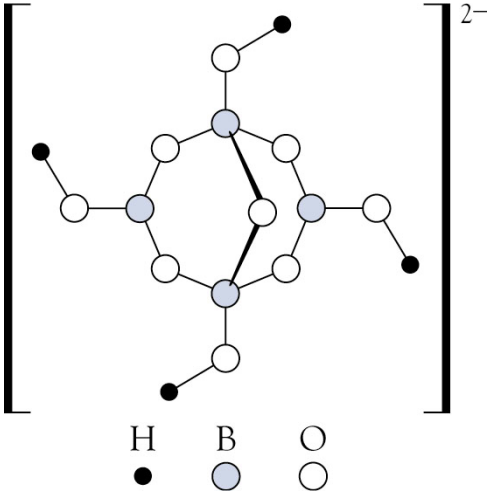
\includegraphics[width=0.5\textwidth]{figures/k13s293Borax.png}
\end{flashcard}

\begin{flashcard}[Struktur]{Tegn strukturen af peroxoborationen}
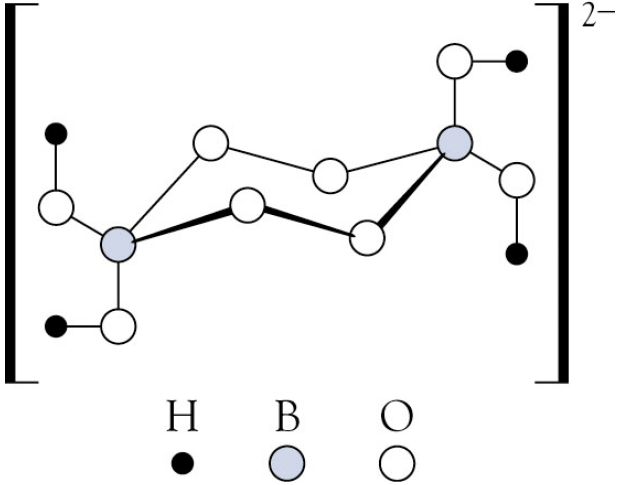
\includegraphics[width=0.5\textwidth]{figures/k13s293Peroxoborat.png}
\end{flashcard}

\begin{flashcard}[Fremstilling]{Opskriv reaktionen for fremstilling af peroxoborationen}
\ce{[B4O5(OH)4]^{2-} + 4H2O2 + 2OH- -> 2[B2(O2)2(OH)4]^{2-} + 3H2O}
\end{flashcard}

\begin{flashcard}[Fremstilling]{Opskriv reaktionen for fremstilling af borcarbid samt reaktionen for fremstilling af titaniumborid}
\ce{2B2O3 + 7C ->[\text{$\Delta$}] B4C + 6CO}\\ \vspace{7pt}
\ce{2TiO2 + B4C + 3C ->[\text{$\Delta$}] 2TiB2 + 4CO}
\end{flashcard}

\begin{flashcard}[Struktur]{Tegn strukturen af diboran}
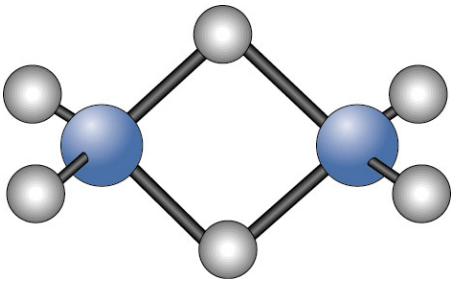
\includegraphics[width=0.5\textwidth]{figures/k13s295Diboran.png}
\end{flashcard}

\begin{flashcard}[Struktur]{Tegn strukturen af pentaboran(9)}
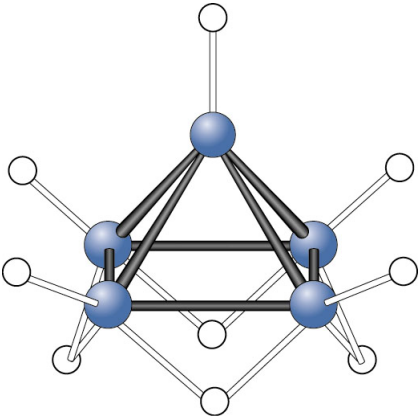
\includegraphics[width=0.5\textwidth]{figures/k13s296Pentaboran.png}
\end{flashcard}

\begin{flashcard}[Struktur]{Tegn strukturen af tetraboran(10)}
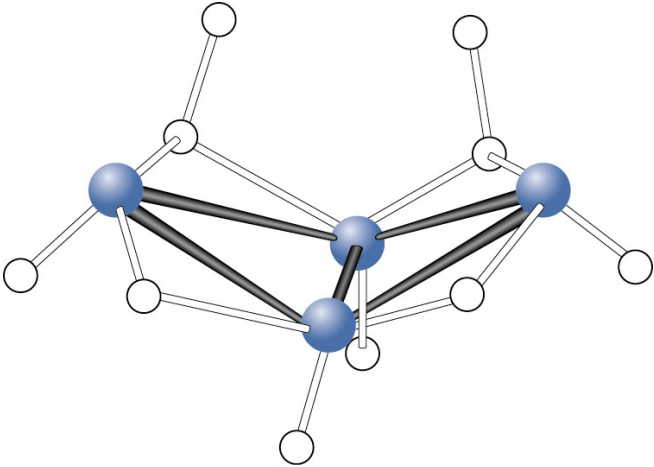
\includegraphics[width=0.7\textwidth]{figures/k13s296Tetraboran.png}
\end{flashcard}

\begin{flashcard}[Fremstilling]{Beskriv fremstillingen af diboran ved hj�lp af et reaktionsskema}
\begin{align*}
\ce{2\OX{rf1,\ox{+3,\ce{B}}}F3 + 6Na\OX{of1,\ox{-1,\ce{H}}} -> \OX{re1,\ox{-3,\ce{B2}}}\OX{oe1,\ox{+1,\ce{H6}}} + 6NaF}
\redox(of1,oe1){\small oxidation}
\redox(rf1,re1)[][-1]{\small reduktion}
\end{align*}
\end{flashcard}

\begin{flashcard}[Fremstilling]{Beskriv fremstillingen af tetraboran og pentaboran med reaktionsskemaer}
\ce{2B2H6 -> B4H10 + H2} \\ \vspace{7pt}
\ce{B4H10 + B2H6 -> 2B5H11 + 2H2}
\end{flashcard}

\begin{flashcard}[Reaktion]{Opskriv diborans reaktion med oxygen og vand}
\ce{B2H6 + 3O2 -> B2O3 + 3H2O}\\ \vspace{7pt}
\ce{B2H6 + 6H2O -> 2H3BO3 +6H2}
\end{flashcard}

\begin{flashcard}[Fremstilling]{Opskriv reaktionen for fremstilling af natriumborhydrid}
\ce{B2H6 + 2NaH -> 2NaBH4}
\end{flashcard}

\begin{flashcard}[Egenskab]{Aluminium metal er amfotert. Opskriv dets reaktion med syre henholdsvis base}
\ce{2Al + 6H+ + 6H2O -> 2[Al(OH2)6]^{3+} + 3H2}\\ \vspace{7pt}
\ce{2Al + 2OH- + 6H2O -> 2[Al(OH)4]- + 3H2}
\end{flashcard}

\begin{flashcard}[Egenskab]{Aluminium(III) i vandig opl�sning er en svag syre p� linje med eddikesyre. Opskriv reaktionen med vand}
\ce{[Al(OH2)6]^{3+} + H2O -> [Al(OH2)5(OH)]^{2+} + H3O+}
\end{flashcard}

\begin{flashcard}[Fremstilling]{Beskriv den industrielle fremstilling af aluminium metal med reaktionsskemaer}
\ce{Al2O3 + 2OH- + 3H2O -> 2[Al(OH)4]-}\\
\ce{2[Al(OH)4]- -> Al2O3\cdot 3H2O(s) + 2OH-}\\
\ce{Al2O3\cdot 3H2O ->[\text{$\Delta$}] Al2O3 + 3H2O}\\
Herefter f�lger elektrolyse af smeltet aluminiumoxid i cryolit
\end{flashcard}

\begin{flashcard}[Fremstilling]{Beskriv den industrielle fremstilling af cryolit med reaktionsskemaer}
\ce{3SiF4 + 2H2O -> 2H2SiF6 + SiO2}\\
\ce{H2SiF6 + 6NH3 + 2H2O -> 6NH4F + SiO2}\\ \vspace{7pt}
\ce{6NH4F + Na[Al(OH)4] + 2NaOH -> Na3AlF6 + 6NH3 + 6H2O}
\end{flashcard}

\begin{flashcard}[Struktur]{Hvilken struktur har \ce{MgAl2O4} henholdsvis \ce{Fe3O4}?}
\ce{MgAl2O4} er en spinel mens \ce{Fe3O4} er en invers spinel
\end{flashcard}